\section{Теоретичні відомості}
\subsection{Метод головних компонент}
Метод головних компонент (Principal component analysis) --- метод, що дозволяє
зменшити розмірність досліджуваної вибірки з мінімальними втратами інформації.
\cite{Aivazyan:1989}

Маємо $m$ об’єктів, з яких треба зняти по $n$ певних властивостей.
На вході в нас є виборки $\vec{X}_k$, кожна з яких відповідає сукупності
властивостей $k$-го об’єкту
\begin{equation*}
  \vec{X}_k = \begin{bmatrix}
    x_k^1  \\
    x_k^2  \\
    \vdots \\
    x_k^n
  \end{bmatrix},
  \qquad k = \overline{1,m}
\end{equation*}
Згрупуємо всі вимірювання в одну матрицю $X$
\begin{equation*}
  X = \begin{bmatrix}
    x_1^1  & x_2^1  & \dots  & x_m^1  \\
    x_1^2  & x_2^2  & \dots  & x_m^2  \\
    \vdots & \vdots & \ddots & \vdots \\
    x_1^n  & x_2^n  & \dots  & x_m^n
  \end{bmatrix}
\end{equation*}

Спочатку нам знадобиться знайти вибіркові середні значення для кожної
властивості
\begin{equation*}
  a_i = \frac{1}{m} \cdot \sum_{k=1}^{m} x_k^i, \qquad i = \overline{1,n}
\end{equation*}
Маємо вектор вибіркових середніх значень
\begin{comment}
\begin{equation*}
  \vec{a} = \begin{bmatrix}
    \frac{1}{m} \sum_{k=1}^{m} x_k^1 \\
    \frac{1}{m} \sum_{k=1}^{m} x_k^2 \\
    \vdots                           \\
    \frac{1}{m} \sum_{k=1}^{m} x_k^n \\
  \end{bmatrix}
\end{equation*}
\end{comment}
\begin{equation*}
  \vec{a} = \begin{bmatrix}
    a_1    \\
    a_2    \\
    \vdots \\
    a_n
  \end{bmatrix}
\end{equation*}

Центруємо отримані дані, що містяться в матриці $X$, віднявши від кожного
стовбця вектор вибіркових середніх $\vec{a}$
\begin{comment}
\begin{equation*}
  \tilde{x}_k^i = x_k^i - a_i,\qquad k = \overline{1,m}, i = \overline{1,n}
\end{equation*}
Кожен стовбець матриці вимірювань прийме вигляд
\begin{equation*}
  \tilde{X}_k
  = \vec{X}_k - \vec{a}
  = \begin{bmatrix}
    x_k^1 - a_1 \\
    x_k^2 - a_2 \\
    \vdots      \\
    x_k^n - a_n
  \end{bmatrix},
  \qquad k = \overline{1,m}
\end{equation*}
Маємо матрицю центрованих вимірювань $\tilde{X}$
\end{comment}
\begin{equation*}
  \tilde{X}
  = \begin{bmatrix}
    \tilde{x}_1^1  & \tilde{x}_2^1  & \dots  & \tilde{x}_m^1  \\
    \tilde{x}_1^2  & \tilde{x}_2^2  & \dots  & \tilde{x}_m^2  \\
    \vdots & \vdots & \ddots & \vdots \\
    \tilde{x}_1^n  & \tilde{x}_2^n  & \dots  & \tilde{x}_m^n
  \end{bmatrix}
  = \begin{bmatrix}
    x_1^1 - a_1  & x_2^1 - a_1  & \dots  & x_m^1 - a_1 \\
    x_1^2 - a_2  & x_2^2 - a_2  & \dots  & x_m^2 - a_2 \\
    \vdots       & \vdots       & \ddots & \vdots      \\
    x_1^n - a_n  & x_2^n - a_n  & \dots  & x_m^n - a_n
  \end{bmatrix}
\end{equation*}

Обчислюємо вибіркову коваріаційну матрицю властивостей.
Вибіркову коваріацію $i$ та $j$ властивості рахуємо за формулою
\begin{equation*}
  \sigma_i^j
  = \frac{1}{m} \cdot \sum_{k=1}^{m} \tilde{x}_k^i \cdot \tilde{x}_k^j
  = \frac{1}{m} \cdot \sum_{k=1}^{m}
    \left[ \left( x_k^i - a_i \right) \cdot \left( x_k^j - a_j \right) \right],
    \qquad i,j = \overline{1,n}
\end{equation*}
Маємо вибіркову коваріаційну матрицю
\begin{equation*}
  K = \begin{bmatrix}
    \sigma_1^1 & \sigma_2^1 & \dots  & \sigma_n^1 \\
    \sigma_1^2 & \sigma_2^2 & \dots  & \sigma_n^2 \\
    \vdots     & \vdots     & \ddots & \vdots     \\
    \sigma_1^n & \sigma_2^n & \dots  & \sigma_n^n \\
  \end{bmatrix}
\end{equation*}
\begin{comment}
\begin{equation*}
  K =
  \begin{bmatrix}
    \frac{1}{m} \cdot \sum_{k=1}^{m} \tilde{x}_k^1 \cdot \tilde{x}_k^1
    &
    \frac{1}{m} \cdot \sum_{k=1}^{m} \tilde{x}_k^1 \cdot \tilde{x}_k^2
    &
    \dots
    &
    \frac{1}{m} \cdot \sum_{k=1}^{m} \tilde{x}_k^1 \cdot \tilde{x}_k^n
    \\
    \frac{1}{m} \cdot \sum_{k=1}^{m} \tilde{x}_k^2 \cdot \tilde{x}_k^1
    &
    \frac{1}{m} \cdot \sum_{k=1}^{m} \tilde{x}_k^2 \cdot \tilde{x}_k^2
    &
    \dots
    &
    \frac{1}{m} \cdot \sum_{k=1}^{m} \tilde{x}_k^2 \cdot \tilde{x}_k^n
    \\
    \vdots & \vdots & \dots & \vdots \\
    \frac{1}{m} \cdot \sum_{k=1}^{m} \tilde{x}_k^n \cdot \tilde{x}_k^1
    &
    \frac{1}{m} \cdot \sum_{k=1}^{m} \tilde{x}_k^n \cdot \tilde{x}_k^2
    &
    \dots
    &
    \frac{1}{m} \cdot \sum_{k=1}^{m} \tilde{x}_k^n \cdot \tilde{x}_k^n
  \end{bmatrix}
\end{equation*}
\end{comment}

Щоб отримувати лише потрібну інформацію, ми хочемо знайти таке ортогональне
лінійне перетворення $L$ вхідної матриці $\tilde{X}$, щоб отримати матрицю
$Y = L \cdot \tilde{X}$, яка має діагональну вибіркову ковариаційну матрицю $K'$
з незростаючими зверху вниз значеннями.
Діагональна вибіркова коваріаційна матриця гарантує той факт, що отримані
значення $Y$ будуть некорельованими.
Рангування значень діагональних елементів матриці $K'$ за величиною дасть більш
наочне уявлення про будову досліджуваних об’єктів, адже діагональні
елементи --- вибіркові дисперсії.
Чим більше дисперсія, тим більше відповідна властивість змінюється від об’єкту
до об’єкту, і тим більше корисної інформації вона нам надає.

Вибіркова коваріаційна матриця $K'$ для $Y = L \cdot \tilde{X}$ має вигляд
\begin{equation*}
  K'
  = L \cdot K \cdot L^*
  = \begin{bmatrix}
    \lambda_1 & 0         & \dots  & 0      \\
    0         & \lambda_2 & \dots  & 0      \\
    \vdots    & \vdots    & \ddots & \vdots \\
    0         & 0         & \dots  & \lambda_n
  \end{bmatrix}
\end{equation*}
З лінійної алгебри відомо, що матриця $L$ складається з координат власних
векторів матриці $K$, а елементи $\lambda_k$ --- її власні числа, які
існують і є невід’ємними через невід’ємну означеність матриці $K$.
Вважаємо, що числа $\lambda_1, \dots, \lambda_n$ впорядковані від більшого до
меншого для зручності подальших дій.
Позначимо власний вектор матриці $K$, що відповідає власному числу $\lambda_k$,
як $\vec{l}_k$. Тоді
\begin{equation*}
  \vec{l}_k
  = \left[ l_k^1, l_k^2, \dots, l_k^n \right],
  \qquad k = \overline{1,n}
\end{equation*}
Матриця $L$ має вигляд
\begin{equation*}
  L = \begin{bmatrix}
    l_1^1  & l_1^2  & \dots  & l_1^n  \\
    l_2^1  & l_2^2  & \dots  & l_2^n  \\
    \vdots & \vdots & \ddots & \vdots \\
    l_n^1  & l_n^2  & \dots  & l_n^n  \\
  \end{bmatrix}
\end{equation*}

Треба зменшити розмірність простору досліджуваних параметрів системи з $n$ до
$p<n$, але при цьому втратити якомога менше відомостей про досліджувані
об’єкти.
Введемо міру інформації, що залишається при зменшенні кількості компонент, що
розглядаються
\begin{equation*}
  I = \frac{\lambda_1 + \dots + \lambda_p}{\lambda_1 + \dots + \lambda_n}
\end{equation*}
Будемо вважати, що діємо продуктивно, тому починаємо обирати з перших
компонент, адже саме вони є найбільш інформативними.
Також бачимо, що інформативність змінюється в межах від $0$
(нічого не дізнаємось) до $1$ (зберегли усю інформацію).

Надалі буде розглядатися матриця головних компонент $Y$
\begin{equation*}
  Y = \begin{bmatrix}
    y_1^1  & y_2^1  & \dots  & y_m^1  \\
    y_1^2  & y_2^2  & \dots  & y_m^2  \\
    \vdots & \vdots & \ddots & \vdots \\
    y_1^p  & y_2^p  & \dots  & y_m^p  \\
    \end{bmatrix}
\end{equation*}
\subsection{Гістограма}

Для подальшого аналізу потрібно здобути щільність розподілу головних компонент.
Оскільки маємо справу з вибіркою і вибірковими характеристиками,
потрібно побудувати гістограму, адже це і є вибіркова характеристика,
що відповідає щільності.

Побудуємо $j$-й стовбець гістограми для виборки з $k$-ї строки матриці $Y$
\begin{equation*}
  h_j^k = \frac{1}{m} \cdot \sum_{i=1}^{m} \indicator{y_i^k \in I_j^k},
  \qquad j = \overline{1, N},
  \qquad k = \overline{1, p}
\end{equation*}
де $I^k$ --- набір напівінтервалів, що розбиває відрізок
$\left[ \min\limits_{i=\overline{1,m}}{y_i^k};
\max\limits_{i=\overline{1,m}}{y_i^k} \right]$ на $N$ рівних частин.
Для вибору $N$ можна скористатися досить відомою формулою Стьорджеса
(Sturges' formula) \cite{Sturges:1926:CCI}
\begin{equation*}
  N = \lfloor \log_2 m \rfloor + 1
\end{equation*}
Маємо матрицю гістограм
\begin{equation*}
  H = \begin{bmatrix}
    h_1^1  & h_2^1  & \dots  & h_N^1  \\
    h_1^2  & h_2^2  & \dots  & h_N^2  \\
    \vdots & \vdots & \ddots & \vdots \\
    h_1^p  & h_2^p  & \dots  & h_N^p
  \end{bmatrix}
\end{equation*}
і напівінтервалів, що відповідають кожному стовбчику кожної гістограми
\begin{equation*}
  I = \begin{bmatrix}
    I_1^1  & I_2^1  & \dots  & I_N^1  \\
    I_1^2  & I_2^2  & \dots  & I_N^2  \\
    \vdots & \vdots & \ddots & \vdots \\
    I_1^p  & I_2^p  & \dots  & I_N^p
  \end{bmatrix}
\end{equation*}

\subsection{Критерій узгодженості Пірсона $\chi^2$}
Гістограма може використовуватися не тільки для графічної інтерпретації
отриманих даних, але й для віднесення вибірки до якогось відомого розподілу.
Відповідь на питання ``Чи дійсно вибірка $y_1^k$, $\dots$, $y_m^k$ має розподіл
$F^k$?'' може надати критерій узгодженості Пірсона.

Розглянемо вектор
\begin{equation*}
    \eta^k
    = \left[ \frac{\nu_1^k - m \cdot \rho_1^k}{\sqrt{m \cdot \rho_1^k}}, \dots,
      \frac{\nu_N^k - m \cdot \rho_N^k}{\sqrt{m \cdot \rho_N^k}} \right]
\end{equation*}
Знайдемо його характеристичну функцію
\begin{equation*}
  \varphi_{\eta^k}\left( \lambda\right)
  = \mean{e^{i \cdot \left( \lambda, \eta^k \right)}},\qquad
  \lambda \in \mathbb{R}^N
\end{equation*}
Для зручності перепозначимо індикатор
\begin{equation*}
  \mathfrak{I}_{i,j}^k = \Indicator{y_i^k \in I_j^k}
\end{equation*}
Подивимось, чому дорівнює скалярний добуток в експоненті
\begin{equation*}
  \begin{split}
    \left( \lambda, \eta^k \right)
    &= \sum_{j=1}^{N} \lambda_j \cdot \frac{\nu_j^k - m \cdot \rho_j^k}{
      \sqrt{m \cdot \rho_j^k}}
    = \sum_{j=1}^{N}\frac{\lambda_j}{\sqrt{m \cdot \rho_j^k}}
      \cdot \sum_{i=1}^{m}\left( \mathfrak{I}_{i,j}^k - \rho_j^k \right) = \\
    &= \sum_{j=1}^{N} \sum_{i=1}^{m}
      \frac{\lambda_j}{\sqrt{m \cdot \rho_j^k}}
      \cdot \left( \mathfrak{I}_{i,j}^k - \rho_j^k \right)
    = \sum_{i=1}^{m} \sum_{j=1}^{N} \lambda_j \cdot
      \frac{\mathfrak{I}_{i,j}^k - \rho_j^k}{\sqrt{m \cdot \rho_j^k}}
  \end{split}
\end{equation*}
Бачимо суму $m$ незалежних однаково розподілених випадкових величин.
Введемо позначення
\begin{equation*}
  \mathfrak{I}_j^k = \Indicator{y_1^k \in I_j^k}
\end{equation*}
А також позначимо новий випадковий вектор
\begin{equation*}
  \zeta^k
  = \left[ \frac{\mathfrak{I}_1^k - \rho_1^k}{\sqrt{m \cdot \rho_1^k}},
    \dots
    \frac{\mathfrak{I}_N^k - \rho_N^k}{\sqrt{m \cdot \rho_N^k}} \right]
\end{equation*}
Тоді скалярний добуток прийме вигляд
\begin{equation*}
    \left( \lambda, \eta^k \right)
    = \sum_{i=1}^{m} \sum_{j=1}^{N} \lambda_j \cdot \zeta_j^k
    = \sum_{i=1}^{m} \left( \lambda, \zeta^k \right)
    = m \cdot \left( \lambda, \zeta^k \right)
\end{equation*}
За рахунок незалежності випадкових величин $\zeta_j^k$ маємо
\begin{equation}\label{eq:cf:eta}
  \varphi_{\eta^k}\left( \lambda\right)
  = \mean{e^{i \cdot \left( \lambda, \eta^k \right)}}
  = \mean{e^{m \cdot i \cdot \left( \lambda, \zeta^k \right)}}
  = \left( \mean{e^{i \cdot \left( \lambda, \zeta^k \right)}} \right)^m
\end{equation}
Розглянемо характеристичну функцію випадкового вектора $\zeta^k$
\begin{equation}\label{eq:cf:zeta}
  \varphi_{\zeta^k}\left( \lambda \right)
  = \Mean{\exp{\left\{ i
    \cdot \sum_{j=1}^{N} \lambda_j \cdot \zeta_j^k \right\}}}
\end{equation}
Легко побачити, що
\begin{equation*}
  \begin{split}
    \left( \lambda, \zeta^k \right)
    = \sum_{j=1}^{N} \lambda_j \cdot \zeta_j^k
    = \sum_{j=1}^{N} \lambda_j
      \cdot \frac{\mathfrak{I}_j^k - \rho_j^k}{\sqrt{m \cdot \rho_j^k}}
    &= \sum_{j=1}^{N} \left(
       \frac{\lambda_j}{\sqrt{m \cdot \rho_j^k}} \cdot \mathfrak{I}_j^k
       - \frac{\sqrt{\rho_j^k} \cdot \lambda_j}{\sqrt{m}} \right) = \\
    &= \sum_{j=1}^{N} \mathfrak{I}_j^k \cdot \left( 
        \frac{\lambda_j}{\sqrt{m \cdot \rho_j^k}}
        - \sum_{l=1}^{N} \frac{\sqrt{\rho_l^k} \cdot \lambda_l}{\sqrt{m}}
      \right)
  \end{split}
\end{equation*}
Тобто характеристична функція \eqref{eq:cf:zeta} приймає вигляд
\begin{equation*}
  \varphi_{\zeta^k}\left( \lambda \right)
  = \Mean{\sum_{j=1}^{N} \mathfrak{I}_j^k
    \cdot \exp{\left\{ \frac{i}{\sqrt{m}} \left(
      \frac{\lambda_j}{\sqrt{\rho_j^k}}
      - \sum_{l=1}^{N} \sqrt{\rho_l^k} \cdot \lambda_l \right) \right\}}}
\end{equation*}
Перепозначимо вираз в круглих дужках
\begin{equation*}
  \mathfrak{z}^k
  = \frac{\lambda_j}{\sqrt{\rho_j^k}}
    - \sum_{l=1}^{N} \sqrt{\rho_l^k} \cdot \lambda_l
\end{equation*}
Математичне очікування індикатора --- ймовірність події, яку він перевіряє.
Отже
\begin{equation*}
  \varphi_{\zeta^k}\left( \lambda \right)
  = \sum_{j=1}^{N} \rho_j^k
    \cdot \exp{\left\{ \frac{i \cdot \mathfrak{z}^k}{\sqrt{m}} \right\}}
\end{equation*}

Якщо розмір вибірки $m$ буде зростати, то характеристична функція $\eta^k$
\eqref{eq:cf:eta} буде поводитись наступним чином
\begin{equation*}
  \begin{split}
    \lim_{m \to \infty} \varphi_{\eta^k}\left( \lambda \right)
    &= \lim_{m \to \infty} \left( 1 + \sum_{k=1}^{N} p_k \cdot \left[
      \exp{\left\{ \frac{i \cdot \mathfrak{z}^k}{\sqrt{m}} \right\}}
      - 1 \right] \cdot \frac{m}{m} \right)^m = \\
    &= \lim_{m \to \infty} \exp{ \left\{ m \cdot \sum_{k=1}^{N} p_k \cdot \left[
      \exp{\left\{ \frac{i \cdot \mathfrak{z}^k}{\sqrt{m}} \right\}}
      - 1 \right] \right\}}
  \end{split}
\end{equation*}
Для $\exp{\left\{ \frac{i \cdot \mathfrak{z}^k}{\sqrt{m}} \right\}}$
використаємо співвідношення
\begin{equation*}
  e^{\alpha} - 1 \approx \alpha + \frac{\alpha^2}{2},\qquad \alpha \ll 1
\end{equation*}
Маємо
\begin{equation*}
  \begin{split}
    \sum_{j=1}^{N} \rho_j^k \cdot \frac{i \cdot \mathfrak{z}^k}{\sqrt{m}}
    &= \sum_{j=1}^{N} \rho_j^k \cdot \frac{i}{\sqrt{m}}
      \cdot \left( \frac{\lambda_j}{\sqrt{\rho_j^k}}
        - \sum_{l=1}^{N} \sqrt{\rho_l^k} \cdot \lambda_l \right) = \\
    &= \frac{i}{\sqrt{m}} \cdot \left(
      \sum_{j=1}^{N} \sqrt{\rho_j^k} \cdot \lambda_j
      - \sum_{l=1}^{N} \sqrt{\rho_l^k} \cdot \lambda_l \right)
    = 0,
  \end{split}
\end{equation*}
\begin{equation*}
  \begin{split}
    \sum_{j=1}^{N} \rho_j^k
      \cdot \left( \frac{i \cdot \mathfrak{z}^k}{\sqrt{m}} \right)^2
      = - \sum_{j=1}^{N} \frac{\rho_j^k}{m}
        \cdot \left( \frac{\lambda_j}{\sqrt{\rho_j^k}}
          - \sum_{l=1}^{N} \sqrt{\rho_l^k} \cdot \lambda_l \right)^2 = \\
      = - \frac{1}{m} \cdot \left[ \sum_{j=1}^{N} \lambda_j
        - \left( \sum_{l=1}^{N} \sqrt{\rho_l^k} \cdot \lambda_l \right)^2
          \right]
  \end{split}
\end{equation*}
Тому
\begin{equation*}
  \begin{split}
    \lim_{m \to \infty} \varphi_{\eta^k}\left( \lambda \right)
    &= \lim_{m \to \infty} \exp{\left\{ -\frac{m}{m \cdot 2}
      \cdot \left[ \sum_{j=1}^{N} \lambda_j
        - \left( \sum_{l=1}^{N} \sqrt{\rho_l^k} \cdot \lambda_l \right)^2
        \right]\right\}} = \\
    &= \exp{\left\{ -\frac{1}{2} \cdot
      \left[ \sum_{j=1}^{N} \lambda_j
        - \left( \sum_{l=1}^{N} \sqrt{\rho_l^k} \cdot \lambda_l \right)^2
        \right] \right\}}
    = e^{-\frac{1}{2} \cdot \left( A^k \lambda, \lambda \right)}
  \end{split}
\end{equation*}
Матриця $A^k$ побудована наступним чином
\begin{equation*}
  A^k
  = \left\| \delta_{ij} - \sqrt{\rho_i^k} \cdot \sqrt{\rho_j^k} \right\|_{i=1}^n
\end{equation*}
Симетричність мариці очевидна, тому треба довести її невід’ємну визначеність,
щоб стверджувати, що вона є коваріаційною.
Для цього візьмемо вектор
\begin{equation*}
  e^k = \left[ \sqrt{\rho_1^k}, \dots, \sqrt{\rho_N^k} \right],\qquad
  \left\| e^k \right\| = 1
\end{equation*}
Тоді бачимо, що
\begin{equation}\label{eq:chi2:quadraticForm}
  \left( A^k \lambda, \lambda \right)
  = \left\| \lambda \right\|^2
    - \left( \lambda, e^k \right)^2
\end{equation}
З нерівності Коші маємо
\begin{equation*}
  \left\| \left( \lambda, e^k \right) \right\|
  \le \left\| \lambda \right\| \cdot \left\| e^k \right\|
  = \left\| \lambda \right\|
\end{equation*}
Тобто матриця є дійсно невід’ємно визначеною і вектор $\eta^k$ розподілений
за нормальним законом з нульовим середнім і коваріаційною матрицею $A^k$.

Для подальших розрахунків розглянемо стандартний гаусівський вектор
як суму випадкових нормально розподілених випадкових величин в стандартному
базисі $\mathbb{R}^N$, який позначимо $\left[ e_1, \dots, e_N \right]$
\begin{equation*}
  \xi = \sum_{j=1}^{N}\xi_j \cdot e_j \sim N\left( \vec{0}, I \right)
\end{equation*}
Згадуємо, що ортогональні перетворення $U$ зберігають відстані, а також
справедливо наступне
\begin{equation*}
  U\xi \sim N\left( 0, U I U^{-1} \right) \sim N\left( \vec{0}, I \right)
\end{equation*}
Також ортонормований базис залишається ортонормованим базисом після
ортогонального перетворення $U$.
Оберемо такий оператор $U$, щоб набір $\left[ e_1, \dots, e_N \right]$ під його
дією перетворився на $\left[ f_1, \dots, f_N \right]$, де
\begin{equation*}
  f_1 = e^k = \left[ \sqrt{\rho_1^k}, \dots, \sqrt{\rho_N^k} \right]
\end{equation*}
Тоді маємо вектор
\begin{equation*}
  U\xi
  = \hat{\xi}
  = \sum_{j=1}^{N} \hat{\xi_j} \cdot f_j \sim N\left( \vec{0}, I \right)
\end{equation*}
Подивимось, який розподіл має наступний вектор
\begin{equation*}
  \Upsilon
  = \sum_{j=2}^{N} \hat{\xi_j} \cdot f_j
  = \hat{\xi} - \hat{\xi_1} \cdot e^k
\end{equation*}
Для цього розглянемо квадратичну форму
\begin{equation*}
  \mean{\left( \Upsilon, \lambda \right)^2}
  = \sum_{j=2}^{N} \left( \lambda, f_j \right)^2
  = \sum_{j=1}^{N} \left( \lambda, f_j \right)^2 - \left( \lambda, f_1 \right)^2
  = \left\| \lambda \right\|^2 - \left( \lambda, e^k \right)^2
  = \left( A^k \lambda, \lambda \right)
\end{equation*}
З рівності \eqref{eq:chi2:quadraticForm} бачимо, що випадкові вектори $\eta^k$
та $\Upsilon$ мають однаковий розподіл.
Отже, розподіли їх норм теж співпадають.
Оскільки сума $N-1$ квадратів незалежних стандартних гаусових випадкових
величин має розподіл Пірсона з $N-1$ ступенями вільності
\begin{equation*}
  \left\| \Upsilon \right\|^2 = \sum_{j=2}^{N} \xi_j^2 \sim \chi_{N-1}^2
\end{equation*}
Маємо
\begin{equation*}
  \left\| \eta^k \right\|
  = \sum_{j=1}^{N}\frac{\left( \nu_j^k - m \cdot \rho_j^k \right)^2}{
    m \cdot \rho_j^k}
  = m \cdot \sum_{j=1}^{N}\frac{\left( h_j^k - \rho_j^k \right)^2}{\rho_j^k}
  \sim \chi_{N-1}^2
\end{equation*}

Останнє співвідношення дає змогу перевіряти належність виборки
$y_1^k$, $\dots$, $y_m^k$ до розподілу $F^k$.
Перевірка виглядає наступним чином.

Розглянемо випадкову величину
\begin{equation}\label{eq:pearson:Rk}
  R^k
  = m \cdot \sum_{j=1}^{N}\frac{\left( h_j^k - \rho_j^k \right)^2}{\rho_j^k}
\end{equation}

Обираємо рівень значущості $\alpha$ для функції розподілу $\chi_{N-1}^2$ і
шукаємо відповідне до кількості ступенів вільності $r_{\alpha}$.
Рівень значущості --- ймовірність помилки першого роду, тобто ймовірність того,
що буде відкинуто вірну гіпотезу
\begin{equation*}
  \probability{\chi_{N-1}^2 \ge r_{\alpha}} = \alpha
\end{equation*}
Якщо $R^k \le r_{\alpha}$, то гіпотеза про те, що вибірка $Y^k$ дійсно має
розподіл $F^k$, приймається.

Розглянемо той випадок, коли ймовірність $\rho_i^k$
відгадана невірно. Повернемося до формули \eqref{eq:pearson:Rk}
\begin{equation*}
  R^k
  = \sum_{j=1}^{N}\frac{\left( \nu_j^k - m \cdot \rho_j^k \right)^2}{m \cdot \rho_j^k}
\end{equation*}
Всі члени суми є невід’ємними. Якщо хоча б один елемент буде завеликим,
то великою буде вся сума. Маємо випадкову величину $\eta$
\begin{equation*}
  \eta
  = \nu_i^k - m \cdot \rho_i^k
  = \sum_{j=1}^{m} \left( \xi_j - \rho_i^k \right),
  \qquad \indicator{y_j^k \in I_i^k} = \xi_j
\end{equation*}
Якщо $\rho_i^k$ вгадано невірно, то воно не дорівнює математичному очікуванню
індикатора. Додамо та віднімемо справжнє математичне очікування
\begin{equation*}
  \eta
  = \sum_{j=1}^{m} \left( \xi_j - \mean{\xi_1} + \mean{\xi_1} - \rho_i^k \right)
  = \sum_{j=1}^{m} \left( \xi_j - \mean{\xi_1} \right)
    + \sum_{j=1}^{m} \left( \mean{\xi_1} - \rho_i^k \right)
\end{equation*}
Останній доданок є просто різницею, помноженою на $m$
\begin{equation*}
  \eta
  = \sum_{j=1}^{m} \left( \xi_j - \mean{\xi_1} \right)
    + m \cdot \left( \mean{\xi_1} - \rho_i^k \right)
\end{equation*}
Поділимо на $\sqrt{m}$, щоб скористатися центральною граничною теоремою
\begin{equation*}
  \frac{\eta}{\sqrt{m}}
  = \frac{1}{\sqrt{m}} \cdot \sum_{j=1}^{m} \left( \xi_j - \mean{\xi_1} \right)
    + \frac{1}{\sqrt{m}} \cdot m \cdot \left( \mean{\xi_1} - \rho_i^k \right)
\end{equation*}
Перший доданок асимптотично має розподіл $N\left( 0, \sigma^2 \right)$, де
$\sigma^2$ --- дисперсія випадкової величини $\xi_1$ для достатньо великих $m$.
Отже, вся сума зростає пропорційно до $\sqrt{m}$
\begin{equation*}
  \frac{\eta}{\sqrt{m}}
  = \frac{1}{\sqrt{m}} \cdot \sum_{j=1}^{m} \left( \xi_j - \mean{\xi_1} \right)
    + \sqrt{m} \cdot \left( \mean{\xi_1} - \rho_i^k \right)
  \sim \sqrt{m} \cdot \left( \mean{\xi_1} - \rho_i^k \right)
\end{equation*}
Тобто зараз $R^k$ буде зростати пропорційно до величини
$m$, і буде великим у порівнянні з $r_{\alpha}$, що призведе до відхилення
невірної гіпотези.

\subsection{Типи вищої нервової діяльності}

Для визначення того, які показники вимірювати і яким чином,
скористуємось відомою класифікацією типів вищої нервової діяльності.

Згідно з Павловим\cite{Pavlov:1923} типи вищої нервової діяльності
характеризуються трьома показниками: сила нервової системи (сильна або слабка),
врівноваженість (врівноважена або неврівноважена)
та рухливість (рухлива або інетртна).
Павлов розглядає 4 комбінації цих показників з 8 можливих:
\begin{enumerate}
  \item Слабка
  \item Сильна та неврівноважена
  \item Сильна, врівноважена та інертна
  \item Сильна, врівноважена та рухлива
\end{enumerate}
Далі ці класи (комбінації) будуть називатися відповідно слабкий,
неврівноважений, інертний та рухливий.
%Щоб віднести людину до того чи іншого класу, існує тест Айзенка.
%Складність полягає в тому, що не дуже часто зустрічаються чисті типи ---
%зазвичай вони змішані.

\subsection{Теппінг-тест (Tapping rate)}

Існують відомі залежності між типом вищої нервової діяльності та зміною
максимального темпу рухів кистю руки з часом.
Протягом 30 секунд людина намагається притримуватися максимально можливого для
себе темпу.
Показники темпу фіксуються через кожні 5 секунд, а далі по 6 отриманим точкам
будується крива темпа руху. \cite{Ilin:2001}

Для тесту можна використовувати ручку (олівець) і папір, або телеграф.
Сучасні технології дозволяють проводити тест за допомогою клавіатури комп’ютера
або екрану планшета.

З олівцем і папіром тест поводиться наступним чином:
\begin{enumerate}
  \item На папері креслиться 6 квадратів
  \item Людина починає ставити якомога більше точок в першому квадраті впродовж
    перших 5 секунд
  \item Коли проходить 5 секунд, потрібно перейти до наступного квадрату і
    ставити точки там
  \item Процедура повторюється до тих пір, доки не пройде 30 секунд --- в кінці
    буде заповнено всі 6 квадратів
\end{enumerate}
Далі підраховується кількість точок в кожному квадраті та малюється ламана, де
горизонтальна вісь відповідає номеру часового проміжку (номеру квадрата), а
вертикальна відповідає кількості точок в квадраті.

Трактуються отримані дані наступним чином:
\begin{enumerate}
  \item Спадна ламана відповідає слабкому типу (рис. \ref{fig:tapping:weak}).
    Вона спадає після перших 5 секунд тесту і не повертається до початкового
    рівня
  \item Ламана, що спочатку зростає, а після 10-15 секунд спадає нижче
    початкового рівня (проміжна між рівною та опуклою) відповідає
    неврівноваженому типу (рис. \ref{fig:tapping:middle}).
  \item Ввігнута ламана відповідає інертному типу
    (рис. \ref{fig:tapping:concave}).
    Вона спочатку спадає, а на 25-30 секундах може зрости до початкового темпу
  \item Опукла ламана відповідає рухливому типу
    (рис. \ref{fig:tapping:movable}).
    Це така ламана, що зростає в перші 10-15 секунд тесту, а після 25-30
    секунд повертається або падає нижче початкового рівня
  \item Також темп може залишатися приблизно на одному рівні протягом
    усього тесту, що є оптимальним для складання іспитів
    (рис. \ref{fig:tapping:flat}).
\end{enumerate}

Оскільки цей тест заснований на вимірюванні витривалості нервової системи людини
за умови максимального навантаження та перевіряє темп реагування (натиснення) на
подразнювачі (внутрішній подразнювач --- команда собі ``треба тиснути''),
було вирішено використовувати відомі вигляди кривих
(рис. \ref{fig:studentBehaviorSimple}) при моделюванні результатів
виконання завдань однакової складності.

\begin{figure}[h]
  \centering
  \begin{subfigure}[b]{0.3\textwidth}
  \resizebox{\textwidth}{!}{\drawHist{chartMovable}}
                \caption{Опукла}
                \label{fig:tapping:movable}
  \end{subfigure}
  \begin{subfigure}[b]{0.3\textwidth}
  \resizebox{\textwidth}{!}{\drawHist{chartMiddle}}
                \caption{Проміжна}
                \label{fig:tapping:middle}
  \end{subfigure}
  \begin{subfigure}[b]{0.3\textwidth}
  \resizebox{\textwidth}{!}{\drawHist{chartFlat}}
                \caption{Рівна}
                \label{fig:tapping:flat}
  \end{subfigure}\\[2ex]
  \begin{subfigure}[b]{0.3\textwidth}
  \resizebox{\textwidth}{!}{\drawHist{chartConcave}}
                \caption{Ввігнута}
                \label{fig:tapping:concave}
  \end{subfigure}
  \begin{subfigure}[b]{0.3\textwidth}
  \resizebox{\textwidth}{!}{\drawHist{chartWeak}}
                \caption{Спадна}
                \label{fig:tapping:weak}
  \end{subfigure}
  \caption{Загальний вигляд залежностей кількості поставлених точок від часу.
  Пунктирна лінія --- кількість точок в перші 5 секунд}
  \label{fig:studentBehaviorSimple}
\end{figure}

Потрібно зауважити, що швидкість розв’язування задач може змінюватися з
досвідом.
Тобто, якщо студент зі слабкою нервовою системою буде тренуватися виконувати
завдяння, то його показники з часом перейдуть на якісно новий рівень.
Щодо студентів з сильною нервовою системою: швидкість не завжди означає якість
виконання завдань.

Мета системи, що буде створено, --- виявляти в автоматичному режимі слабкі
місця студентів  при виконанні завдань, а потім надавати поради викладачам
практичних занять.
Наприклад, тим, що надто швидко втомлюються, потрібно розв’яювати якомога
більше базових завдань, що не є складними, але розв’язок яких повинен бути
на рівні рефлексів.
Студентам, які поспішають, буде наказано ретельно коментувати у письмовій
формі хід своїх думок, щоб вгамуватися та підвищити свою уважність.

При використанні теппінг-тесту в якості сировини виникає потреба у
диференціюванні студентів за знанням галузей, до яких відносяться задачі.
Тобто, якщо завдання однакової складності, то вони можуть перевіряти знання
лише в тому випадку, коли відносяться до різних тем, які студент може знати або
ні.
В обох випадках студенту може знадобитися час на те, щоб згенерувати відповідь
або принаймні спробувати.
З’являється складність: в межах одного завдяння у студента виникає кілька
підзадач, кількість яких залежить від методу розв’язання, що він обере,
і неможливо наперед вирахувати всі можливі способи вирішення тієї чи іншої
проблеми.

\subsection{Адаптованість}
Якщо розглянути ламані на рис. \ref{fig:studentBehaviorSimple} і поєднати їх,
то отримаємо щось схоже на рис. \ref{fig:studentBehaviorCommon}, де на осі
абсцис цифрами 1, 2, 3 і 4 позначено початок відповідно ввігнутої, опуклої,
проміжної та спадної кривої.

\begin{figure}[h]
  \centering
  %\resizebox{\textwidth}{!}{\drawHist{chartCommon}}
  %\drawHist{chartCommon}
  \includestandalone[]{tikz/studentBehaviorCommon}
  \caption{Загальна картина активності}
  \label{fig:studentBehaviorCommon}
\end{figure}

З рисунку видно, що в людей з сильною нервовою системою спостерігається ефект
адаптованості --- так зване ``друге дихання'', чого немає у власників слабкої.
Також бачимо, що крива прямого типу може бути отримана, якщо зменшити впадину
між двома горбами на графіку --- примусити швидше працювати механізми, що
збуджують адаптованість.

Щоб почати моделювання результатів тестів на основі відомих ламаних
результатів теппінг-тесту, потрібно змоделювати результати самого
теппінг-тесту.
Форма графіку, що зображено на рис. \ref{fig:studentBehaviorCommon},
спочатку нагадує синусоїду, але як його продовжити, якщо
скористатися тим припущенням, що далі крива не буде зростати?

\subsection{Відпочинок як процес Пуассона}

Була спроба моделювати поведінку студента простим методом: в якості параметра
брати його початковий ритм, а потім віднімати від нього реалізації процесу
Пуассона з інтенсивністю $c \cdot t$ у відповідні проміжки часу.
Тобто, було припущення, що в студента є певний ритм роботи, а його змушує
сповільнюватися потреба у відпочинку, яка зростає з часом.
Ідея розглядати кількість розв’язаних задач як процес Пуассона виявилася
поганою як математично, так і ідеологічно: був дуже великий розкид значень,
та взагалі хотілось би розглядати вирішення завдань як результат цілеспрямованої
роботи студента, а не випадковий процес.

Для $c = \frac{1}{5}$ було отримано як досить цікаві для використання результати
(рис. \ref{fig:poisson:strange}), так і не дуже (рис. \ref{fig:poisson:wrong}).
Моделювання проводилося за допомогою пакету NHPoisson мови програмування R.
\begin{figure}[h]
  \centering
  \begin{subfigure}[b]{0.4\textwidth}
    \resizebox{\textwidth}{!}{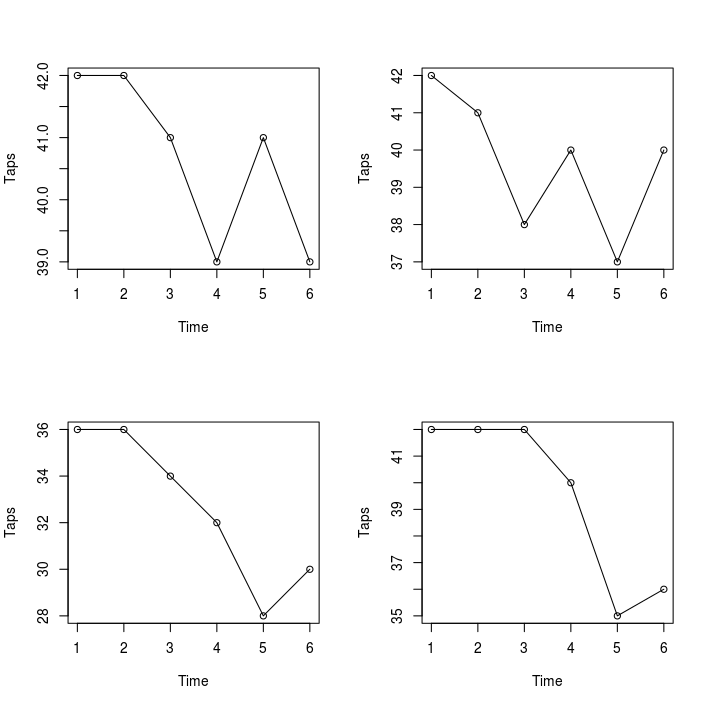
\includegraphics{code/strange}}
    \caption{Задовільні результати}
    \label{fig:poisson:strange}
  \end{subfigure}
  \begin{subfigure}[b]{0.4\textwidth}
    \resizebox{\textwidth}{!}{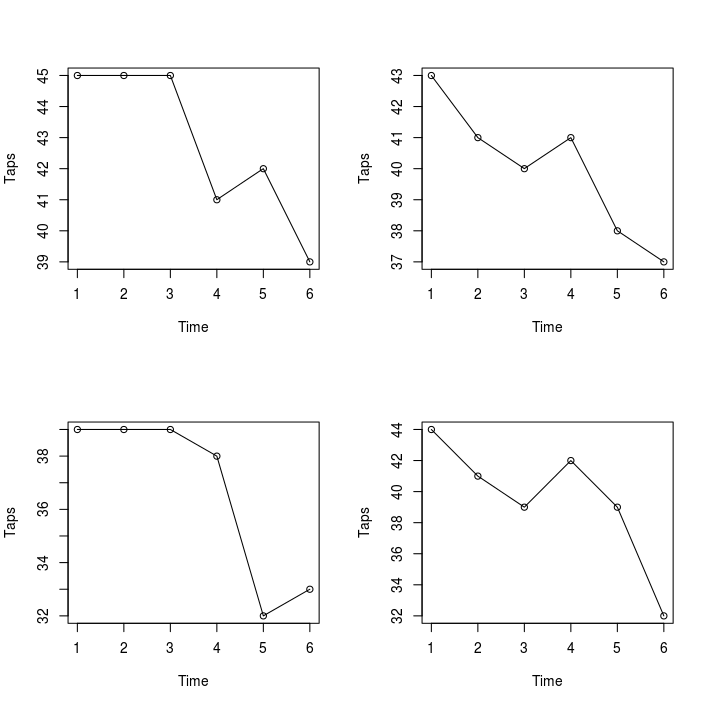
\includegraphics{code/wrong}}
    \caption{Незадовільні результати}
    \label{fig:poisson:wrong}
  \end{subfigure}
  \caption{Моделювання результатів теппінг-тесту}
  \label{fig:tapping:poisson}
\end{figure}

З рис. \ref{fig:tapping:poisson} видно, що серед гідних для подальшого аналізу
ламаних трапляються ті, що мають занадно великі перепади.
Також за допомогою такого підходу не вийде змоделювати різноманітні вигляди
майже рівної кривої, адже мінімальне значення кількості ``відпочинків'' є
нульовим.
Якщо до цієї моделі додати шум (наприклад, замість гаусового використовувати
незалежні випадкові, що розподілені за законом Бернуллі) для вирішення проблеми
від’ємних значень, то це створить додаткові завеликі стрибки ламаної
(рис. \ref{fig:poisson:bernoulli})
\begin{figure}[h]
  \centering
  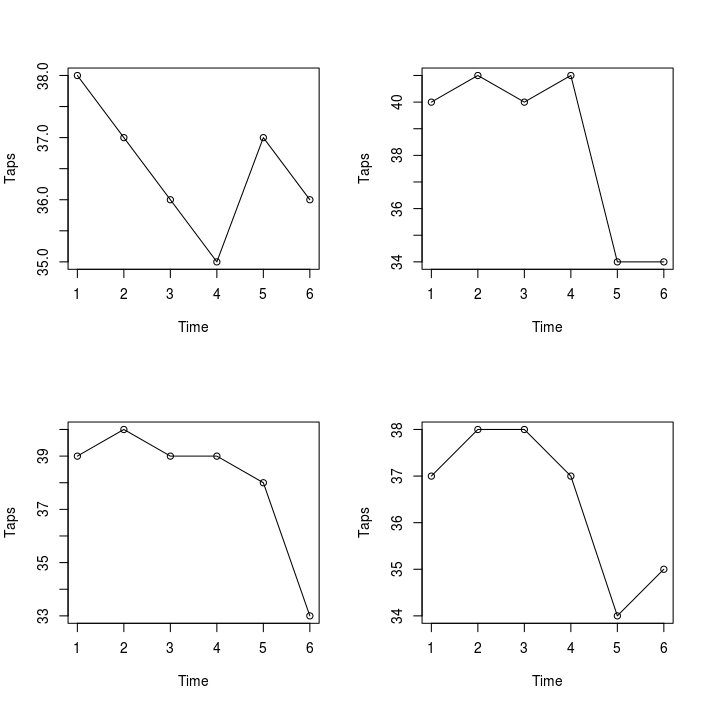
\includegraphics[width=9cm]{code/bernoulli}
  \caption{Результати з додаванням центрованих Бернуллієвських випадкових
  величин з параметрами $\left( 2, 0.5 \right)$}
  \label{fig:poisson:bernoulli}
\end{figure}

Дана модель демонструє себе як просту, але не завжди адекватну: її результати
потрібно фільтрувати.
Тим не менш, нестандартні результати можна трактувати як ненормальну поведінку
студента, якому потрібно пояснити, що під час контрольної роботи або екзамену
він повинен бути більш зібраним та повністю концентруватися тій на роботі, що
потрібно виконати.

\subsection{Гідравліка}

Для моделювання результатів теппінг-тесту постулюємо такі правила:
\begin{enumerate}
  \item У студента є певний запас енергії для виконання роботи, який з часом
    вичерпується, а накопичується лише після відпочинку (зміну роду занять)
  \item Коли студент працює на повну силу, він втрачає енергію
  \item Чим менше енергії залишається, тим повільніше вона витрачається
  \item Адаптованість --- поява додаткової енергії
\end{enumerate}

Це нагадує процес витікання рідини при змінному напорі води --- коли її рівень
в посудині змінюється.
Якщо рівень рідини в цистерні змінюється достатньо повільно, можна скористатися
наступним співвідношенням \cite{Sheypak:2007}
\begin{equation}\label{eq:hydraulics}
  A \cdot dh = - \mu \cdot S \cdot \sqrt{h} \cdot dt
\end{equation}
$A$ --- площа поперечного перерізу посудини на висоті $h$ від отвору;\\
$S$ --- площа поперечного перерізу отвору внизу посудини;\\
$dh$ --- зміна висоти рідини за час $dt$;\\
$\mu$ --- константа, яка включає в себе прискорення вільного падіння,
стиснення рідини біля отвору тощо, але в поточній задачі її сенс, звісно,
буде іншим.

Моментальна швидкість зміни об’єму рідини буде рахуватися за формулою
\begin{equation}\label{eq:hydrodynamics:volumeChange}
  \upsilon\left( t \right)
  = \frac{dV}{dt} = \frac{d\left( h \cdot A \right)}{dt}
\end{equation}

Коли площі поперечних перерізів цистерни та отвору постійні, маємо таке рівняння
для зміни висоти рідини
\begin{equation*}
  \dot{h}
  = - \mu \cdot \frac{S}{A} \cdot \sqrt{h},
  \qquad  \dot{A} = \dot{S} = 0
\end{equation*}
Отримуємо лінійне диференційне рівняння з розділеними змінними
\begin{equation*}
  h^{-\frac{1}{2}} \cdot dh
  = - \mu \cdot \frac{S}{A} \cdot dt
\end{equation*}
Інтегруємо в межах від $t_0 = 0$ до $t$
\begin{equation*}
  \int\limits_{h_0}^{h\left( t \right)} h^{-\frac{1}{2}} \; dh
  = - \mu \cdot \frac{S}{A} \cdot \int\limits_0^t dt
\end{equation*}
Та маємо розв’язок
\begin{equation}\label{eq:fluid:height}
  h\left( t \right)
  = \left( \sqrt{h_0}
    - \frac{\mu}{2} \cdot \frac{S}{A} \cdot t \right)^2
\end{equation}
Швидкість зміни об’єму
\begin{equation}\label{eq:fluid:velocity}
  \upsilon\left( t \right)
  = A \cdot \dot{h}
  = - \mu \cdot S \cdot \sqrt{h_0}
    \cdot \left( 1 - \frac{\mu \cdot S}{2 \cdot \sqrt{h_0}} \cdot t \right)
\end{equation}
Оскільки вважається, що студент працює максимально продуктивно, а це означає,
що швидкість спорожнення цистерни максимальна, то з розв’язків
бачимо, що це досягається тоді, коли площа отвору $S$ максимальна.
Оскільки вона не може бути більша за $A$, то залишається лише прирівняти
$A = S$.
Оскільки рівень рідини повинен зменшуватися повільно, то висота $h_0$ повинна
бути набагато більшою за $S$ --- маємо витікання рідини з трубки.
В такому разі залежність висоти рідини від часу \eqref{eq:fluid:height} приймає
наступний вигляд
\begin{equation*}
  h\left( t \right)
  = \left( \sqrt{h_0}
    - \frac{\mu}{2} \cdot t \right)^2
\end{equation*}

Щоб враховувати адаптованість, потрібно додати ще одне джерело рідини,
з якого вона буде виливатися в досліджувану цистерну.

Нехай $V_2$ --- об’єм додаткової цистерні, тоді $\upsilon_2$ --- швидкість
зміни об’єму рідини, що в ній знаходиться.
Відомо, що
\begin{enumerate}
  \item Нехай швидкість витікання води з основної цистерни не може перевищувати
    початкове значення $\upsilon\left( 0 \right)$ (умовилися з вигляду
    результатів теппінг-тесту)
  \item В певний момент часу $\tau$ перетікання води зупиняється
  \item В момент часу $\tau$ в основній посудині знову знаходиться така
    кількість рідини, що була спочатку
    \begin{equation*}
      \int\limits_{0}^{\tau} \upsilon_2 \; dt
      = \int\limits_{0}^{\tau} \upsilon \; dt
    \end{equation*}
\end{enumerate}

З останнього факту легко знайти об’єм додаткової рідини $V_a$ звичайним
інтегруванням
\begin{equation*}
  V_a
  = - \int\limits_{0}^{\tau} \upsilon \; dt
  = \mu \cdot S \cdot \sqrt{h_0}
    \cdot \left( 1 - \frac{\mu \cdot S}{4 \cdot \sqrt{h_0}} \cdot \tau \right) \cdot \tau
\end{equation*}

Бачимо, що на даний момент важко сказати ще щось окрім того, що коли
додаткова рідина поступає нерівномірно (не одразу активується механізм
адаптованості), то
\begin{enumerate}
  \item Якщо швидкість витікання води з основної цистерни не перевищує початкове значення через те, що її висота дорівнює $h_0$ і вона фізично не може містити
    більше рідини, ніж спочатку, то площа отвору $S$ повинна бути меншою за площу перерізу посудини $A$, інакше неможливо буде вливати додаткову рідину таким чином,
    щоб її швидкістю можна було знехтувати
  \item Друга цистерна повинна мати регульовану площу отвору, щоб була можливість моделювати опуклі ламані
\end{enumerate}

Використаємо рівняння \eqref{eq:hydraulics}, щоб підрахувати зміну площі отвору,
яка повинна бути для підтримання постійної швидкості зміни об’єму протягом
певного часу $\tau$ (позначення ті ж самі, але використаємо результати для
другої цистерни)
\begin{equation}\label{eq:hydrodynamics:varSquare}
  \begin{cases}
    \dot{h}         &= - \mu \cdot \frac{S}{A} \cdot \sqrt{h} \\
    \dot{\upsilon}  &= 0
  \end{cases} \Rightarrow
  \begin{cases}
    \dot{h}  &= - \mu \cdot \frac{S}{A} \cdot \sqrt{h} \\
    \ddot{h} &= 0
  \end{cases},
  \qquad \dot{A} = 0
\end{equation}
Об’єднаємо систему рівнянь в одне
\begin{equation*}
  \frac{d\left( S \cdot \sqrt{h} \right)}{dt}
  = 0
\end{equation*}
Диференціюємо добуток. Це не складно, але буде використано далі
\begin{equation}\label{eq:hydrodynamics:valuableResult}
  \dot{S}
  = - \frac{S}{2 \cdot h}
    \cdot \dot{h}
\end{equation}
Маємо залежність $S$ від $h$
\begin{equation}\label{eq:hydrodynamics:varSolutionSh}
  S\left( h \right) = S_0 \cdot \sqrt{\frac{h_0}{h}}
\end{equation}
Тобто, швидкість зміни висоти рідини дорівнює
\begin{equation*}
  \dot{h} = - \mu \cdot \frac{S_0}{A_0} \cdot \sqrt{h_0}
\end{equation*}
Швидкість зміни об’єму рідини, як нескладно здогадатися з
\eqref{eq:fluid:velocity}, рахується за формулою
\begin{equation*}
  \upsilon
  = - \mu \cdot S_0 \cdot \sqrt{h_0}
\end{equation*}

Скористуємось \eqref{eq:hydrodynamics:valuableResult}, щоб знайти
залежність висоти від часу, адже нам потрібно знати, скільки рідини повинно
бути у другій цистерні
\begin{equation*}
  2 \cdot \frac{\dot{S}}{S}
  = - \frac{\dot{h}}{h}
\end{equation*}
Застосуємо \eqref{eq:hydrodynamics:varSquare}
\begin{equation*}
  2 \cdot \frac{\dot{S}}{S}
  = \frac{\mu \cdot S \cdot \sqrt{h}}{A \cdot h}
\end{equation*}
Розділяємо змінні та згадуємо розв’язок рівняння
\eqref{eq:hydrodynamics:varSolutionSh} відносно $\sqrt{h}$
\begin{equation*}
  2 \cdot \sqrt{h_0} \cdot S_0
    \cdot S^{-3} \cdot dS
  = \frac{\mu}{A} \cdot dt
\end{equation*}
Після інтегрування в межах від $0$ до $\tau$ Маємо розв’язок
\begin{equation*}
  S\left( \tau \right)
  = S_0
    \cdot \left[ 1 - \mu
      \cdot \frac{S_0}{A \cdot \sqrt{h_0}} \cdot \tau\right]^{- \frac{1}{2}}
  = \frac{S_0}{\sqrt{1 - \mu
      \cdot \frac{S_0}{A \cdot \sqrt{h_0}} \cdot \tau}}
\end{equation*}
Автоматично з \eqref{eq:hydrodynamics:varSolutionSh} отримали
\begin{equation*}
  h\left( \tau \right)
  = h_0 \cdot \left[ 1 - \mu
      \cdot \frac{S_0}{A \cdot \sqrt{h_0}} \cdot \tau \right]
\end{equation*}
Маємо залежності між параметрами другої цистерни для побудови ламаної рівного
типу.
Залишилося розв’язати задачу для змінної швидкості, щоб будувати опуклі ламані.

Далі потрібно врахувати такі факти:
\begin{enumerate}
  \item Площа отвору додаткової цистерни не може перевищувати площу перерізу
    основної, бо це не має сенсу
  \item Площа отвору додаткової цистерни не може перевищувати площі свого
    перерізу, адже це теж не має сенсу
\end{enumerate}
Сформулюємо обмеження математично
\begin{equation*}
  \begin{cases}
    S_2 &\le A_2 \\
    S_2 &\le A \\
    S   &\le A
  \end{cases}
\end{equation*}
